% arara: pdflatex: { shell: yes }
% arara: bibtex
% arara: pdflatex: { shell: yes }
% arara: pdflatex: { shell: yes }

\documentclass[conference, 10pt, final, a4paper, oneside, twocolumn]{IEEEtran}
\usepackage{cite}
\usepackage{amsmath,amssymb,amsfonts}
\usepackage{algorithmic}
\usepackage{graphicx}
\usepackage{textcomp}
\usepackage{xcolor}
\usepackage{pgfplots, pgfplotstable, tikzscale, standalone}
\usepackage{siunitx}
\usepackage[hidelinks]{hyperref}
\pgfplotsset{width=10cm,compat=1.15}

\pgfplotsset{
    cycle list/.define={marks}{
        every mark/.append style={solid,fill=\pgfkeysvalueof{/pgfplots/mark list fill}},mark=*\\
        every mark/.append style={solid,fill=\pgfkeysvalueof{/pgfplots/mark list fill}},mark=square*\\
        every mark/.append style={solid,fill=\pgfkeysvalueof{/pgfplots/mark list fill}},mark=triangle*\\
        every mark/.append style={solid,fill=\pgfkeysvalueof{/pgfplots/mark list fill}},mark=diamond*\\
        every mark/.append style={solid,fill=\pgfkeysvalueof{/pgfplots/mark list fill}},mark=x\\
    },
}

\def\BibTeX{{\rm B\kern-.05em{\sc i\kern-.025em b}\kern-.08em
    T\kern-.1667em\lower.7ex\hbox{E}\kern-.125emX}}

\begin{document}

\title{Parallel Image Processing}
\author{
    \IEEEauthorblockN{Lorenzo Fasol}
    \IEEEauthorblockA{\textit{University of Trento}\\
    Trento, Italy \\
    Student ID: 227561 \\
    lorenzo.fasol@studenti.unitn.it}
    \and
    \IEEEauthorblockN{Alessandro Iepure}
    \IEEEauthorblockA{\textit{University of Trento}\\
    Trento, Italy \\
    Student ID: 228023 \\
    alessandro.iepure@studenti.unitn.it}
    \and
    \IEEEauthorblockN{Riccardo Minella}
    \IEEEauthorblockA{\textit{University of Trento}\\
    Trento, Italy \\
    Student ID: 227326 \\
    riccardo.minella@studenti.unitn.it}
}
\maketitle

\begin{abstract}
    This report explores parallel image processing algorithms using shared and %
    distributed memory paradigms, along with GPU acceleration. After developing %
    a baseline serial implementation, the algorithm is parallelized using OpenMP, %
    MPI, and CUDA, focusing on convolution-based image filtering for edge detection. %
    Experiments are conducted on a heterogeneous HPC cluster, analyzing performance %
    and scalability. Through theoretical analysis and practical experimentation, %
    this report provides insights into the performance characteristics of parallel %
    image processing algorithms and their scalability across different architectures.
\end{abstract}

\section{Introduction}

Image processing, a fundamental task in computer vision and digital imaging, %
involves manipulating and enhancing digital images to extract useful information %
or to improve their visual quality. In many real-world applications, such as medical %
imaging, video processing, and remote sensing, the performance and efficiency of %
such algorithms are crucial for timely and accurate results. With the %
ever-increasing size and complexity of image data, there is a growing need for %
efficient parallel algorithms to handle the computational demands of this kinds %
of tasks.

The objective of this project was to explore and implement parallel image %
processing algorithms using shared and distributed memory paradigms and GPU accelerators. %
Specifically, we focused on parallelizing image filtering operations, which are %
commonly used for tasks such as noise reduction, edge detection, and image enhancement. %
We implemented and optimized a convolution-based image filtering %
algorithm to detect edges, which applies a filter kernel to each pixel in the %
input image to produce the corresponding pixel in the output image.

We began by developing a serial implementation of the algorithm %
and subsequently parallelized it using OpenMP for shared memory systems, MPI %
for distributed memory systems, and CUDA to harness the power of GPU cores. The parallel %
algorithms were designed to distribute the computational workload efficiently %
among available threads or processes, leveraging the capabilities of modern %
multi-core CPUs, distributed computing clusters and co-processors.

To ensure the correctness and effectiveness of the parallel implementations, %
appropriate boundary-handling strategies were employed to handle edge pixels %
during the convolution operation.\\
The project also analyzed performance and optimizations, including %
evaluating the speedup achieved by the parallel algorithms for different numbers %
of threads or processes.

Overall, this project aimed to provide a comprehensive understanding of parallel %
image filtering algorithms, their implementation, and their performance characteristics %
under different configurations. Through theoretical analysis and practical %
experimentation, we sought to gain insights into the scalability, %
efficiency, and adaptability of parallel image processing techniques.

\section{Implementation}

The baseline algorithm implemented starts by reading an input image from disk. The %
image is then processed by applying padding around the perimeter. This is done to %
ensure that the output image has the same dimensions as the input image after the %
convolution is computed. In our implementation, we have chosen to use zero-padding %
as the boundary-handling strategy. This decision was made based on several factors, %
including simplicity and computational efficiency. While other techniques such as %
mirror padding or wrapping around the image could also be considered, we opted %
for zero-padding due to its minimal impact on performance and its ability to %
preserve the overall structure of the image. By focusing on a single boundary-handling %
strategy, we can more effectively analyze and compare the performance and output %
quality of our parallel image filtering algorithms.
After the convolution is computed, the output image is saved to disk and the elapsed %
time is printed. The latter considers only the convolution operation %
and not the time spent in I/O operations. This is also the performance metric %
we used to evaluate the speedup achieved by the different parallel algorithms. %
The convolution is based on a simple nested loop structure, %
where the filter kernel is applied to each pixel in the input image to produce the %
corresponding pixel in the output image. In our implementation, %
we have chosen to use a simple 3x3 filter kernel for edge detection. 

The serial implementation of the algorithm does verbatim what has been described so far. 

The shared memory parallel implementation uses OpenMP to distribute the computational %
workload among available threads. It does so by introducing parallel regions in the %
padding and convolution operations. The number of threads are set at runtime using the %
\texttt{OMP\_NUM\_THREADS} environment variable.

The distributed memory parallel implementation uses MPI to divide the computational %
workload among all available processes. The trick here is to divide the input image into %
equal-sized chunks and pad them using the neighbors data. To achieve the correct %
padding, the input image is first scattered to all processes, then each one sends %
and receives the top and bottom rows to and from its neighbors. On the reconstructed %
local image we apply the convolution as usual and the results are gathered at the end. 

The GPU parallel implementation uses CUDA to harness the power of GPU cores. The %
kernel is stored on the GPU's constant memory and the input image is copied to %
the device memory after loading it from disk. Padding is achieved by copying the %
input image to a larger array on the device memory. This operation is done in a %
separate CUDA kernel from the convolution operation. The latter is computed %
in parallel by a grid of threads, where each thread computes the convolution of %
a single pixel in the output image. The results are then copied back to the host %
memory in order to be saved to disk. Execution times are measured via CUDA events %
for an accurate value.

\section{Experiments and System Description}

For our experiments, we conducted performance evaluations on the University's HPC %
cluster. Depending on the version of the algorithm executed and the resources required, %
the computing node(s) used changed. The cluster is composed of an heterogeneous set of nodes, %
each with different hardware. Multiple runs were performed for each version of the algorithm, %
and the results were averaged to obtain a more reliable estimate of the performance.

Software wise, all nodes in the cluster run CentOS Linux 7 and the code was compiled %
using the GNU Compiler Collection 9.1.2 (GCC) for the sequential and OpenMP %
implementations, MPICH 3.2 (MPICC) for MPI and the NVIDIA CUDA Compiler 11.3 (NVCC). %

All tests were performed on the same input image, Fig. \ref{fig:inputImage}, with a resolution of %
2560x1920 and 3 color channels per pixel. We chose this image because it is a standard %
test card used in television broadcasting and it contains a variety of patterns and %
colors that are useful for testing edge detection algorithms. The image was also chosen %
because it is relatively large, which allows us to better analyze the performance of our %
parallel algorithms. Image operations are performed %
with the STB Image library, which is a simple library to load and save images %
from files. The library is written in C and is able to load and save images in a %
variety of formats, including JPEG, PNG, BMP, and TGA. Our code works with any %
image as long as it is in one of the supported formats and - for the parallel versions only - %
the height of the image is a multiple of the number of processes or threads.

\begin{figure}
    \centering
    
\includegraphics[width=0.4\textwidth]{../../tvTest.png}
    \caption{\label{fig:inputImage}Philips PM5544 Test card, the input image for the experiments.}
\end{figure}

After experimenting with different block sizes in the CUDA version, we found that %
increasing the block size did not result in any significant performance improvement. %
This is likely because the input image is relatively small, and the overhead of %
launching a large number of threads outweighs any potential benefits. As a result, %
we decided to stick with a block size of 32 which is CUDA's maximum value in our %
setup.

\section{Results and Conclusions}

\begin{table}[!t]
    \renewcommand{\arraystretch}{1.3}
    \caption{\label{table:results}Results of the experiments - Execution times.}
    \centering
    \begin{tabular}{c|c|c|c|c}
        \hline
        \bfseries  & \bfseries Cores & \bfseries Time [\SI{}{\milli\second}] & \bfseries Speedup [$\times$] & \bfseries Efficiency [$\%$]\\
        \hline
        Sequential & - & 758 & 1.00 & 100\\
        \hline
                & 2  & 397 & 1.91  & 95.55\\
                & 4  & 200 & 3.79  & 94.75\\
        OpenMP & 8  & 104 & 7.27  & 90.81\\
                & 16 & 56  & 13.62 & 85.10\\
                & 32 & 33  & 22.74 & 71.06\\
                & 64 & 31  & 24.72 & 38.62\\
        \hline
                & 2  & 415 & 1.83  & 91.33\\
                & 4  & 257 & 2.95  & 73.64\\
        MPI    & 8  & 151 & 5.02  & 62.75\\
                & 16 & 116 & 6.52  & 40.72\\
                & 32 & 100 & 7.58  & 23.69\\
                & 64 & 92  & 8.27  & 12.92\\
        \hline
        CUDA   & - & 10 & 75.80 & - \\
        \hline
    \end{tabular}
\end{table}

OpenMP and MPI versions were tested multiple times each with a different amounts
of threads and processes, respectively. On the other hand, the sequential and CUDA %
versions were tested only once. The results of three runs were averaged to obtain %
a more reliable estimate of the performance. The speedup was calculated as the %
ratio between the execution time of the sequential version and the execution time %
of the parallel version. The efficiency was calculated as the ratio between the %
speedup and the number of threads or processes. The results are shown in Table \ref{table:results}. %

\begin{figure}%
    \centering
    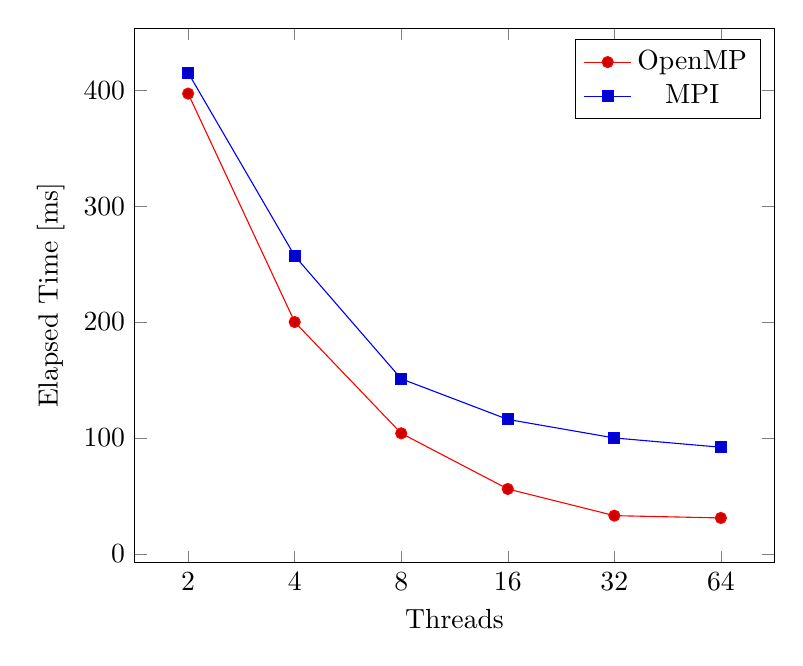
\begin{tikzpicture}%
        \begin{axis}[
                width={0.8\linewidth},
                xlabel={Threads},
                ylabel={Elapsed Time [ms]},
                xtick=data, % Use data points as x-axis ticks
                xticklabels={2, 4, 8, 16, 32, 64}, % Set the x-axis tick labels
                cycle multiindex* list={
                    color list
                        \nextlist
                    marks
                        \nextlist
                },
                xmode=log, % Set x-axis mode to normal
            ]
        
            \addplot
                coordinates {
                    (2, 397)
                    (4, 200)
                    (8, 104)
                    (16, 56)
                    (32, 33)
                    (64, 31)
                };
    
            \addplot
                coordinates {
                    (2, 415)
                    (4, 257)
                    (8, 151)
                    (16, 116)
                    (32, 100)
                    (64, 92)
                };
                
            \legend{OpenMP, MPI}
        \end{axis}
    \end{tikzpicture}
    \caption{\label{fig:plotTime}Comparison graph by number of cores}
\end{figure}
\begin{figure}
    \centering
    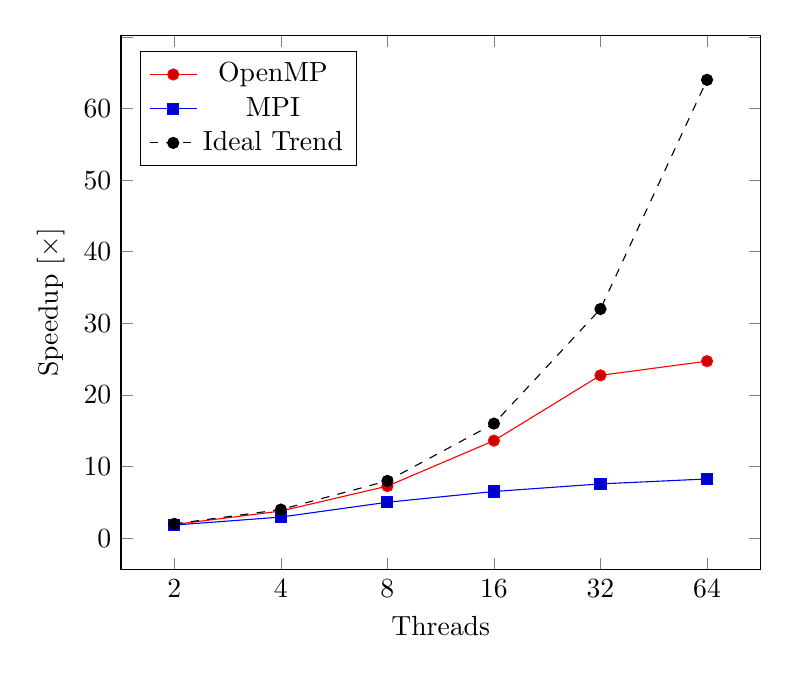
\begin{tikzpicture}%
        \begin{axis}[
                width={0.8\linewidth},
                xlabel={Threads},
                ylabel={Speedup [$\times$]},
                xtick=data, % Use data points as x-axis ticks
                xticklabels={2, 4, 8, 16, 32, 64}, % Set the x-axis tick labels
                yticklabels={-10, 0, 10, 20, 30, 40, 50, 60}, % Set the x-axis tick labels
                cycle multiindex* list={
                    color list
                        \nextlist
                    marks
                        \nextlist
                },
                xmode=log, % Set x-axis mode to normal
                legend pos=north west, % Place the legend on the top right
            ]
        
            \addplot
                coordinates {
                    (2, 1.91)
                    (4, 3.79)
                    (8, 7.27)
                    (16, 13.62)
                    (32, 22.74)
                    (64, 24.72)
                };
    
            \addplot
                coordinates {
                    (2, 1.83)
                    (4, 2.95)
                    (8, 5.02)
                    (16, 6.52)
                    (32, 7.58)
                    (64, 8.27)
                };

            \addplot[dashed, mark=*, mark options={solid}] % BEGIN: Add dashed style to the ideal plot
            coordinates {
                (2, 2)
                (4, 4)
                (8, 8)
                (16, 16)
                (32, 32)
                (64, 64)
            }; % END: Add dashed style to the ideal plot
                
            \legend{OpenMP, MPI, Ideal Trend}
        \end{axis}
    \end{tikzpicture}
    \caption{\label{fig:plotSpeedup}Speedup graph by number of cores}
\end{figure}
\begin{figure}
    \centering
    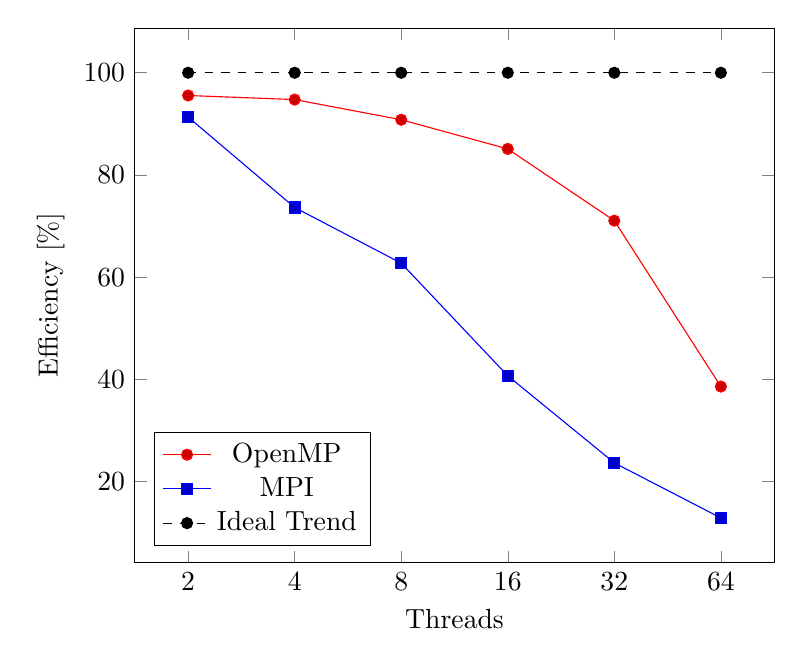
\begin{tikzpicture}%
        \begin{axis}[
                width={0.8\linewidth},
                xlabel={Threads},
                ylabel={Efficiency [\%]},
                xtick=data,
                xticklabels={2, 4, 8, 16, 32, 64},
                cycle multiindex* list={
                    color list
                        \nextlist
                    marks
                        \nextlist
                },
                xmode=log,
                legend pos=south west,
            ]
        
            \addplot
                coordinates {
                    (2, 95.55)
                    (4, 94.75)
                    (8, 90.81)
                    (16, 85.10)
                    (32, 71.06)
                    (64, 38.62)
                };
    
            \addplot
                coordinates {
                    (2, 91.33)
                    (4, 73.64)
                    (8, 62.75)
                    (16, 40.72)
                    (32, 23.69)
                    (64, 12.92)
                };

            \addplot[dashed, mark=*, mark options={solid}]
                coordinates {
                    (2, 100)
                    (4, 100)
                    (8, 100)
                    (16, 100)
                    (32, 100)
                    (64, 100)
                };
                
            \legend{OpenMP, MPI, Ideal Trend}
        \end{axis}
    \end{tikzpicture}
    \caption{\label{fig:plotEfficiency}Efficiency graph by number of cores}
\end{figure}

The experimental results demonstrate the performance characteristics of different %
parallelization techniques for the image processing algorithm. The sequential %
implementation serves as the baseline. Assuming ideal conditions, parallel execution %
times should decrease linearly as the number of cores increase. However, our experiment %
demonstrates that this is not always the case. 

Comparing the execution times, we can see that both OpenMP %
and MPI decrease as the number of cores increases, as shown in Fig. \ref{fig:plotTime}. %
Around 16 cores, the execution times tend to stabile due to Amdahl's Law. Increasing %
the number of cores can reduce the execution time only as long as the %
sequential fraction remains a significant portion of the total time. %
Once it becomes negligible compared to the optimized %
parallel time, further increases in cores will not lead to significant %
additional improvements in the overall time.

Analyzing the results on OpenMP, from 32 to 64 %
cores, the efficiency drops significantly as is observable in Fig. \ref{fig:plotEfficiency}. %
Similarly, the MPI implementation shows a more pronounced drop between 8 and 64 %
processes. This is likely due to increased overhead and resource contention, which %
diminishes the returns in speedup.
Discussing the speedup, OpenMP adheres to the ideal trend up to 32 cores before %
stabilizing. On the other hand, MPI exhibits limited speedup starting from 8 %
cores, remaining constant thereafter. This trend is also evident in Fig. \ref{fig:plotSpeedup}. %
The CUDA implementation, achieves the highest speedup. However the %
resulting efficiency is not directly comparable to the one from the other %
CPU-based implementations in this experiment.

Given the techniques explored, architectures leveraging GPU acceleration, as %
demonstrated in the CUDA implementation, offer the highest speedup, making them %
particularly effective for image processing tasks.

Overall, our findings provide insights into the effectiveness and limitations of %
different parallelization techniques for image processing algorithms. Future %
research could explore optimization strategies to address scalability issues and %
further leverage GPU acceleration for improved efficiency. The experimental results %
underscore the importance of choosing the appropriate parallelization technique %
based on the characteristics of the algorithm and the underlying hardware %
architecture, enabling researchers and developers to make informed decisions to %
optimize performance and address computational challenges in image processing %
tasks.

\section{Project Contributions and Reproducibility}

This report is the result of a collaborative effort between the authors. All decisions %
were discussed, agreed on and developed together. Each author focussed mainly on:
\begin{itemize}
    \item \textbf{Lorenzo Fasol}:
        \begin{itemize}
            \item Sequential version
            \item OpenMP version
            \item CUDA version
        \end{itemize}
    \item \textbf{Alessandro Iepure}:
        \begin{itemize}
            \item Sequential version
            \item MPI version
        \end{itemize}
    \item \textbf{Riccardo Minella}:
        \begin{itemize}
            \item Sequential version
            \item OpenMP version
            \item MPI version
        \end{itemize}
\end{itemize}
The report was co-authored by all of us. All source codes for the various algorithm %
implementations, along with the scripts used for the experiments and other assets, %
are available in the project's GitHub repository at the following link %
\url{https://github.com/aleiepure/Parallel-final}. The repository also contains %
a PDF copy of this document and the \LaTeX{} source code.


\nocite{*}
\IEEEtriggeratref{5}
\bibliographystyle{IEEEtran}
\bibliography{IEEEabrv,assets/bibliography.bib}

\end{document}